\documentclass{uwstat572}
\usepackage{amsmath}
\usepackage{color}
\usepackage{subfigure}
\usepackage{graphicx}

%%\setlength{\oddsidemargin}{0.25in}
%%\setlength{\textwidth}{6in}
%%\setlength{\topmargin}{0.5in}
%%\setlength{\textheight}{9in}

\renewcommand{\baselinestretch}{1.5} 


\bibliographystyle{plainnat}

\begin{document}
%%\maketitle

\begin{center}
  {\LARGE Bayesian Lasso}\\\ \\
  {Annelise Wagner \\ 
    Department of Statistics, University of Washington Seattle, WA, 98195, USA
  }
\end{center}

\begin{abstract}
  The Bayesian Lasso, building on the interpretation of Tibshirani, places Laplace priors on linear regression coefficients to allow for Bayesian approaches to parameter and error estimation. An efficient Gibbs sampler allows for quick computation and may be extended to other forms of penalized regression.
\end{abstract}

TODO: Hoff edits, full conditionals, integration of $\tau$, check convergence, anything in ALLCAPS

\section{Introduction}\label{Introduction}
Regression problems are an extremely common class of approaches to finding linear relationships (or more complex relationships) between a vector of $p$ explanatory variables, $\mathbf{x}$, and a response variable $\mathbf{y}$. The straight forward approach to these problems, even introduced at the most basic level of statistics, is ordinary least squares (OLS) regression. GIVE EXAMPLES OF PROBLEMS SOLVED VIA OLS

OLS regression is fairly well understood, allowing for estimates of regression coefficients, prediction, and error estimation. Despite this, ordinary least squares has a number of problems. Correlation between $\mathbf{x}$ variables may conflate their relationship with $\mathbf{y}$, resulting in biased estimates of regression coefficients. CITE SOMETHING HERE

Another problem that is becoming increasingly common with the prevalence of large data sets, a researcher may not know which of the $\mathbf{x}$ variables are truly related to $\mathbf{y}$, and may have $p$ explanatory variables when only $p'<p$ of them drive the relationship in $\mathbf{y}$. While the relationship between some regressors and $\mathbf{y}$ should be null, \cite{seeger2008bayesian} shows us that OLS will tend to fit all regression coefficients with at least non-zero value, as this will usually produce minor decreases in the squared error.

This takes the problem of finding the best regression coefficients, and introduces a second problem of model selection. For small problems, a total of $2^p$ possible models exist and may be full explored and evaluated according to some information criterion such as AIC or BIC. For a problem like assessing DNA microarray data, where thousands or tens of thousands of data points are collected for tens or hundreds of people, individually assessing models becomes impossible.

Gene expression data is a great example of the problem the Lasso seeks to solve. Many of the variables in $\mathbf{x}$ are not related to the response. This introduces the need for two similar ideas, selection and shrinkage. A method is required that will either select which estimates will be non-zero, or an alternative view is that it needs to shrink estimates to zero (as a means of selecting non-zero eestimates). 

In the case of the gene expression data, \cite{ishwaran2005spike} chose a Bayesian approach akin to a constrained optimization problem known as spike and slab priors was used. EXPLAIN SPIKE AND SLAB HERE

Another form of penalized regression, the Least Absolute Shrinkage and Selection Operator (Lasso), limits the $L_1$ norm of coefficients to produce zero estimates for coefficients. This same idea can be found in signal processing, where Basis Pursuit seeks to select from many different waveforms by penalizing their $L_1$ norms as can be seen in the work by \cite{chen2001atomic}.

One early shortcoming of the Lasso was a lack of estimation of variability. Simple solutions, such as bootstrap sampling, can easily be demonstrated to have problems overestimating the number of zero components as shown by \cite{kyung2010penalized}. In fact, it was shown by \cite{shao1996bootstrap} that these estimates are not even consistent as sample sizes increase. 

One different approach at assessing the variability of $\beta$ estimates, used by \cite{fan2001variable}, produce point estimates of variability via a correction to the sandwich estimator (often used in OLS when one believes the model may be misspecified).

The Bayesian Lasso builds on the idea originally proposed by \cite{tibshirani1996regression}, of treating the Lasso estimates as least squares estimates with Laplace prior distributions placed on regression parameters. By taking advantage of a scale mixture of normals representation of the Laplace distribution an effective Gibbs sampler can be created to produce credible intervals of regression coefficient estimates.

\section{Background and Methods}
Linear regression assumes that we have some vector of responses, $\boldsymbol{y}$, which depend linearly on some covariates, $\boldsymbol{X}$. Formally, accounting for an error term, we wish to fit the model \[
\boldsymbol{y} = \mu \boldsymbol{1}_n + \boldsymbol{X}\boldsymbol{\beta}+\boldsymbol{\epsilon}
\] where $\boldsymbol{y}$ is an $n \times 1$ vector, $\mu$ is the mean of $\boldsymbol{y}$, $\boldsymbol{X}$ is a matrix of regressors (typically standardized), and $\boldsymbol{\epsilon}$ is a vector of independent and identically distributed zero mean normal variables with an unknown variance. For the sake of this discussion we will assume that the $\boldsymbol{y}$ has zero mean ($\mu=0$), noting that in practice this can be easily achieved by subtracting the sample mean estimate from $\mathbf{y}$.

What is of interest is the regression coefficients, $\boldsymbol{\beta}$. These can be used for prediction when new values of regressors are given, or they may be of interest for their interpretation on the effects of certain regressor values on the dependent $\boldsymbol{y}$. Irrespective of the use, there are a number of approaches to finding the regressor coefficients. One familiar method, ordinary least squares, seeks to minimize least squares error\[
\min_{\boldsymbol{\beta}} \hspace{.1cm} (\boldsymbol{y}-\boldsymbol{X}\boldsymbol{\beta})^T(\boldsymbol{y}-\boldsymbol{X}\boldsymbol{\beta}).
\] While OLS estimates are a straight-forward and simple approach, Section~\ref{Introduction} details some of the shortcomings of this method.

Penalized regression takes a similar approach, trying to minimize the square error of predicted values, but with further constraints on regression coefficients. One form of penalization, known as bridge regression, takes the form  \[
\min_{\boldsymbol{\beta}}  \hspace{.1cm} (\boldsymbol{y}-\boldsymbol{X}\boldsymbol{\beta})^T(\boldsymbol{y}-\boldsymbol{X}\boldsymbol{\beta})+\lambda\sum_{j=1}^p|\beta_j|^q
\] for some $q\geq0$. The cases where $q=1$ (Lasso Regression) and $q=2$ (Ridge Regression) have appealing and better understood properties. INSERT ORIGINAL REFERENCE FOR RIDGE AND BRIDGE REGRESSION

The more desirous property of the Lasso is its ability to produce sparse estimates of parameters. It accomplishes this task by restricting solutions onto an $L_1$ 'ball' around the origin. This is more obvious from the dual formulation, 
\begin{align*}
\min_{\boldsymbol{\beta}}  \hspace{.1cm} &(\boldsymbol{y}-\boldsymbol{X}\boldsymbol{\beta})^T(\boldsymbol{y}-\boldsymbol{X}\boldsymbol{\beta})\\
\text{subject to} \hspace{.1cm}&\sum_{j=1}^p|\beta_j|\leq r
\end{align*}
for some $r$ determined by $\lambda$. Figure~\ref{LassoPlot} adapted from \cite{park2008bayesian}, shows how this penalization compares to a Ridge Regression, Bridge Regression with $q=2$ which restricts solutions onto an $L_2$ ball.

\begin{figure}\label{LassoPlot}
  \centering
    \subfigure[Lasso $L_1$ restriction]{
      \centering
      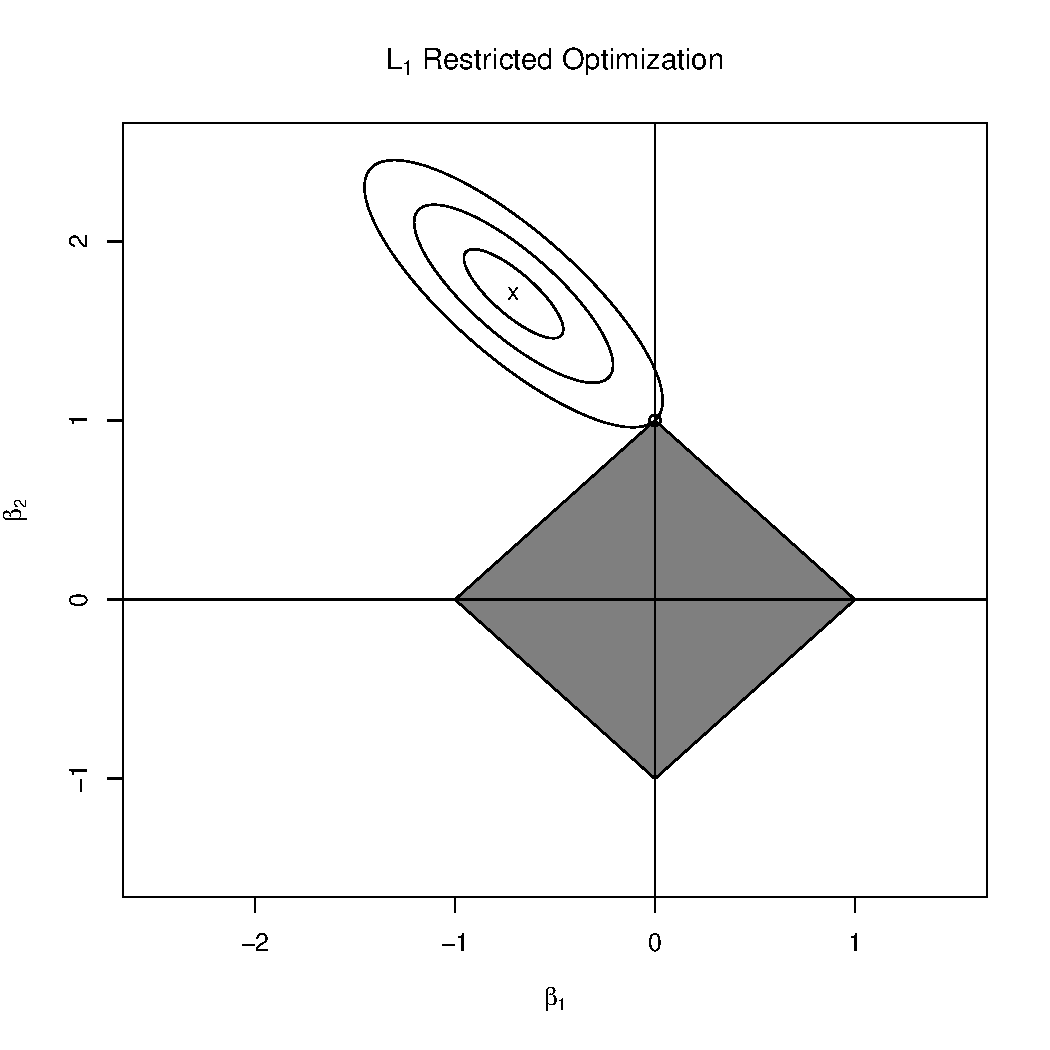
\includegraphics[width=0.45\textwidth]{LassoPlot1.pdf}
    }
    \subfigure[Ridge Regression $L_2$ restriction]{
      \centering
      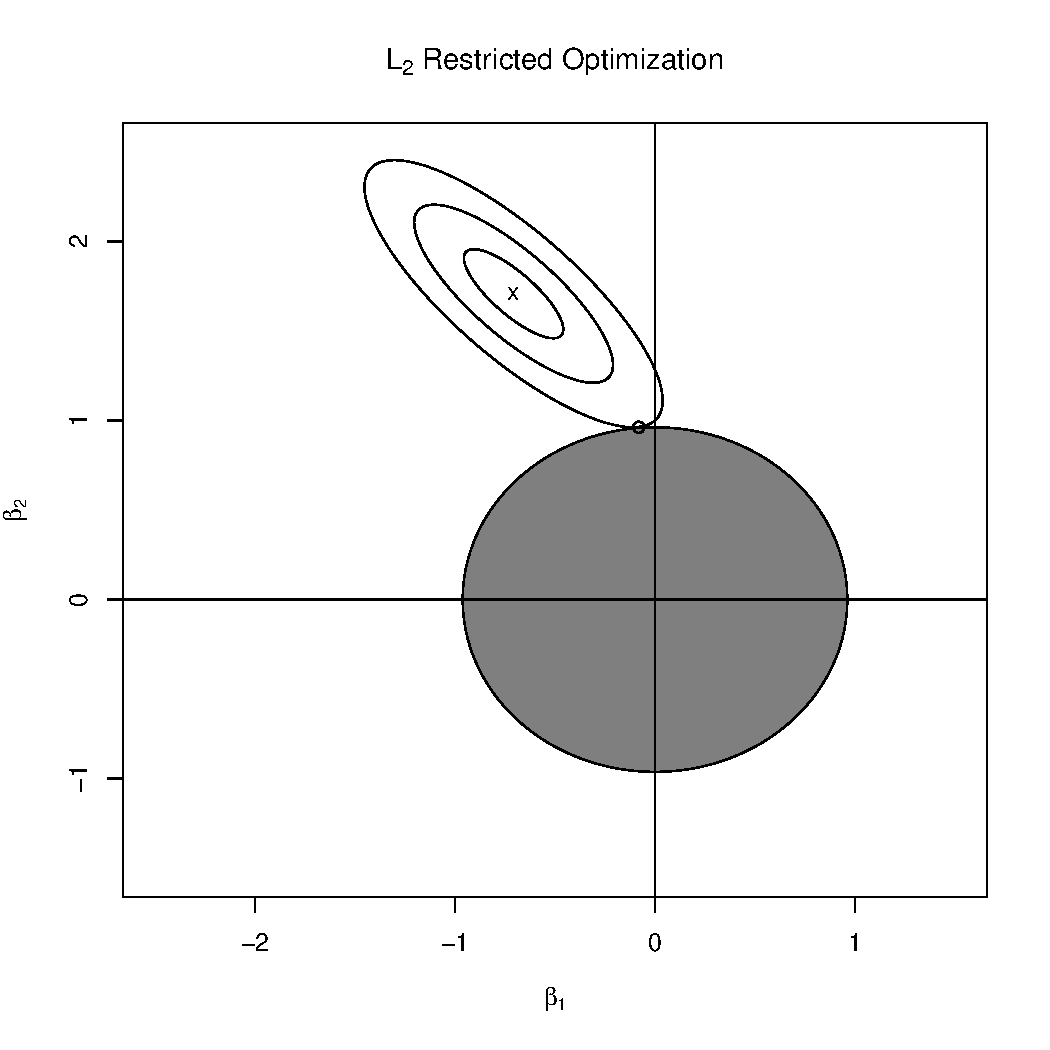
\includegraphics[width=0.45\textwidth]{LassoPlot2.pdf}
    }
  \caption{With an OLS estimate found at $\times$, the ovals represent increasing levels of squared error. In either case we seek a minimal estimate within the restricted shaded region, which will occur at the border of the restricted region (provided $\times$ lies outside). This example illustrates the tendency for Lasso estimates (left) to be driven to 0, compared with Ridge Regression estimates (right) which are close to but not exactly 0 for $\beta_1$.}
\end{figure}

For this reason we are most interested in the Lasso. The standard form representation, for some penalty weight $\lambda \geq 0$, has the form \[
\min_{\boldsymbol{\beta}}  \hspace{.1cm} (\boldsymbol{y}-\boldsymbol{X}\boldsymbol{\beta})^T(\boldsymbol{y}-\boldsymbol{X}\boldsymbol{\beta})+\lambda\sum_{j=1}^p|\beta_j|.
\] In the Lasso original derivation it was noted that these estimates can be equivalently viewed as posterior modes of minimal squared error estimates, when independent Laplace priors are placed on the $\boldsymbol{\beta}$s as suggested by \cite{tibshirani1996regression}.

The Bayesian Lasso, in keeping with Tibshirani's original interpretation, places independent Laplace (or double exponential) distributions on the parameters. Specifically, prior density \[
\pi(\beta|\sigma^2)=\prod_{j=1}^p\frac{\lambda}{2\sqrt{\sigma^2}}e^{-\lambda |\beta_j|/\sqrt{\sigma^2}}
\] is placed on each parameter, which results in a unimodal posterior. The need for a unimodal posterior is more thoroughly addressed in Section~\cite{unimodal}.

\subsection{Prior Distributions}
In keeping with our normal errors being independent and identically distributed Normals, then the response vector is distributed as follows, \[
\mathbf{y}|\mu,\mathbf{X},\boldsymbol\beta,\sigma^2 \sim \text{N}_n(\mu \mathbf{1}_n+\mathbf{X}\boldsymbol\beta,\sigma^2\mathbf{I}_n), \] but again noting that the vector $\mathbf{y}$ should be centered, resulting in $\mu=0$. Alternatively, an independent flat prior on $\mu$ can be used without affecting conjugacy of relevant variables.

The regression parameters $\boldsymbol\beta$, conditioned on their variance estimates $\tau_1^2,...,\tau_p^2$, are given a normal prior, \[ 
\boldsymbol\beta|\sigma^2,\tau^2_1,...,\tau^2_p\sim\text{N}_p(\mathbf{0}_p,\sigma^2\mathbf{D}_\tau),\] with \[ \mathbf{D}_\tau=\text{diag}(\tau_1^2,...,\tau^2_p) \] which is not the double exponential prior intended. To arrive at the desired Laplace distribution, the representation found in \cite{andrews1974scale} allows us to express the Laplace distribution as a scale mixture of normal distributions, \[ \frac{a}{2}e^{-a|z|}=\int^\infty_0
\frac{1}{\sqrt{2\pi s}}e^{-z^2/(2s)}\frac{a^2}{2}e^{-a^2s/2}ds.\] We can then integrate out $\tau^2_1,...,\tau^2_p$ to arrive at the desired distribution, \[ \pi(\boldsymbol\beta|\sigma^2)=\prod^p_{j=1}\frac{\lambda}{2\sqrt{\sigma^2}}e^{-\lambda|\beta_j|/\sqrt{\sigma^2}}, \] which is a Laplace prior. 

The variance $\sigma^2$ can be given an inverse gamma prior distribution (while maintaining conjugacy), but the treatment by \cite{park2008bayesian} instead uses an improper prior, $1/\sigma^2$. 

The variances of $\boldsymbol\beta$, $\tau_1^2,...,\tau_p^2$, are given independent distributions of the form, \[ \tau^2_j \sim \frac{\lambda^2}{2}e^{-\lambda^2\tau^2_j/2}d\tau^2_j.\] 

\subsubsection{$\boldsymbol\beta$ Conditioning on $\sigma^2$}\label{unimodal}
Again it is worth noting that conditioning $\boldsymbol\beta$ on $\sigma^2$ produces a unimodal joint distribution, while independent Laplace priors on $\boldsymbol\beta$ do not have ths trait which can cause convergence problems in the Gibbs sampler. This is most obvious when comparing the joint distribution of $\mathbf{y}$ and $\boldsymbol\beta$. Conditioned on $\sigma^2$ as presented this join has the property, \[
\pi(\mathbf{y},\boldsymbol\beta|\mathbf{X},\sigma^2) \propto \exp{\left(\frac{||\mathbf{y}-\mathbf{X}\boldsymbol\beta||_2}{\sigma^2}+\frac{\lambda ||\boldsymbol\beta||_1}{\sigma^2}\right)}
\] and we can see that taking the logarithm and maximizing gives us exactly the formulation of the Lasso, as $\sigma^2$ doesn't figure into the maximum (over $\lambda$). If we instead express the $\boldsymbol\beta$ as being independent of $\sigma^2$ we end up with \[
\pi(\mathbf{y},\boldsymbol\beta|\mathbf{X},\sigma^2) \propto \exp{\left(\frac{||\mathbf{y}-\mathbf{X}\boldsymbol\beta||_2}{\sigma^2}+\lambda ||\boldsymbol\beta||_1\right)}.
\] This then produces different results for different values of $\sigma^2$ which can (but won't always) lead to bimodality as was shown in the toy example presented by \cite{park2008bayesian}. This is not a necessary condition, and only added to aid convergence.

\subsection{Full Conditionals}
With our priors properly defined, we are then able to sample consecutively from the full conditional distributions of $\boldsymbol\beta$, $\sigma^2$, and $\tau^2_1,...,\tau^2_p$. First defining the matrix $\mathbf{A}=\mathbf{X}^T\mathbf{X}+\mathbf{D}_\tau^{-1}$ for simplification, \[
\boldsymbol\beta|\mathbf{y},\mathbf{X},\sigma^2,\boldsymbol\tau^2 \sim \text{N}_p(\mathbf{A}^{-1}\mathbf{X}^T\mathbf{y},\sigma^2\mathbf{A}^{-1}) \]. The full conditional of the variance is, \[ \sigma^2|\mathbf{y},\mathbf{X},\boldsymbol\beta,\boldsymbol\tau^2 \sim \text{InvGamma}\left(\alpha'=\frac{n-1}{2}+\frac{p}{2},\beta'=(\mathbf{y}-\mathbf{X}\boldsymbol\beta)^T(\mathbf{y}-\mathbf{X}\boldsymbol\beta)+\frac{\boldsymbol\beta\mathbf{D}_\tau^{-1}\boldsymbol\beta}{2}\right). \] And lastly the full conditionals of the coefficient variances $\tau^2_1,...,\tau^2_p$ are independent, with \[
\frac{1}{\tau_j^2} | \boldsymbol\beta, \sigma^2, \lambda \sim \text{InvGaussian}\left(\mu'=\sqrt\frac{\lambda^2\sigma^2}{\beta_j^2}, \lambda'=\lambda^2\right). \] We can then produce a Gibbs sampler by consecutively sampling each of these distributions.

As an aside, if we are interested in keeping $\mu$ in the model, we may simply give it a uniform prior which produces a full coditional that is $\text{N}(\bar{y},\sigma^2/\sqrt{n})$ which can be worked into the Gibbs sampler.

\subsection{Empirical Bayesian Selection of $\lambda$}
One point that has yet to be addressed is the selection of the hyperparameter $\lambda$. A typical approach such as cross-validation is suitable for many applications, but the Bayesian approach taken by \cite{park2008bayesian} allows us to take advantage of the Monte Carlo EM algorithm proposed by \cite{casella2001empirical}. Here, we start with $\lambda^{(0)}$ based on the ordinary least squares estimates \[ 
\lambda^{(0)}=\frac{p\sqrt{\hat\sigma^2_{LS}}}{\Sigma^p_{j=1}|\hat\beta_j^{LS}|} 
\] which is then updated after a run of the Gibbs sampler according to \[ 
\lambda^{(k)}=\sqrt\frac{2p}{\Sigma^p_{j=1}E_\lambda[\tau^2_j|\mathbf{y}]}
\] by replacing the expectation with an average from the Gibbs sample. 

\section{Results}
Assessing a penalized regression can be difficult, and with real world problems no underlying truth is known to compare selected models against. In the context of the Bayesian Lasso, we are most concerned with comparing this approach with the standard Lasso. As will also prove relevant, we also compare this approach with Bridge Regression. 

Estimate paths are an informative tool with any penalized regression, looking at how estimates change over varying levels of penalization. Also of interest are the credible intervals of estimates under constant penalization, which will be studied under the marginal maximum likelihood penalty on $\lambda$.

THIS NEEDS WORK!

\subsection{Data Set}
The algorithm found herein has been tested on the same data used by \cite{efron2004least}. This data comprises $n=442$ diabetes patients observed over a one year period. The regression variables comprise of patient age, sex, body mass index, average blood pressure, and six blood serum measurements such as good and bad cholesterol. These were then looked at as linear predictors of the response, a quantitative measure of diabetes progression at the end of the one year observation period.

It is worth noting here that the specifics of the data set are not of interest. The discussion here is only focused on the effectiveness of the algorithm and we avoid making any quality judgments of the efficacy of our models in the context of the original data.

\subsection{Assessing the Gibbs Sampler}
When working with any MCMC approach it is important to step back and consider the effectiveness of the sampling technique. One thing that concerned me early on was the use of successive Gibbs samples, with no comments on the efficacy of such an approach.

To this end, results were assessed using the CODA package by \cite{codapackage}, which can be used the find diagnostics of an MCMC approach. More specifically, the effective sample sizes were of particular interest.

Following the approach used in the original work, samples of size 10,000 were taken from the Gibbs sampler, after a burn in period of 1,000 samples. After repeated resamplings it was found that the fifth covariate, blood serum triglyceride levels, had an effective sample size approximately 40\%-60\% the size of the sample. The cause for this became readily apparent when looking to Figure~\ref{Var5} which shows a significant correlation at low lags. While other variables also displayed some similar issues, triglyceride levels presented the most extreme and consistent case.

\begin{figure}\label{Var5}
  \centering
    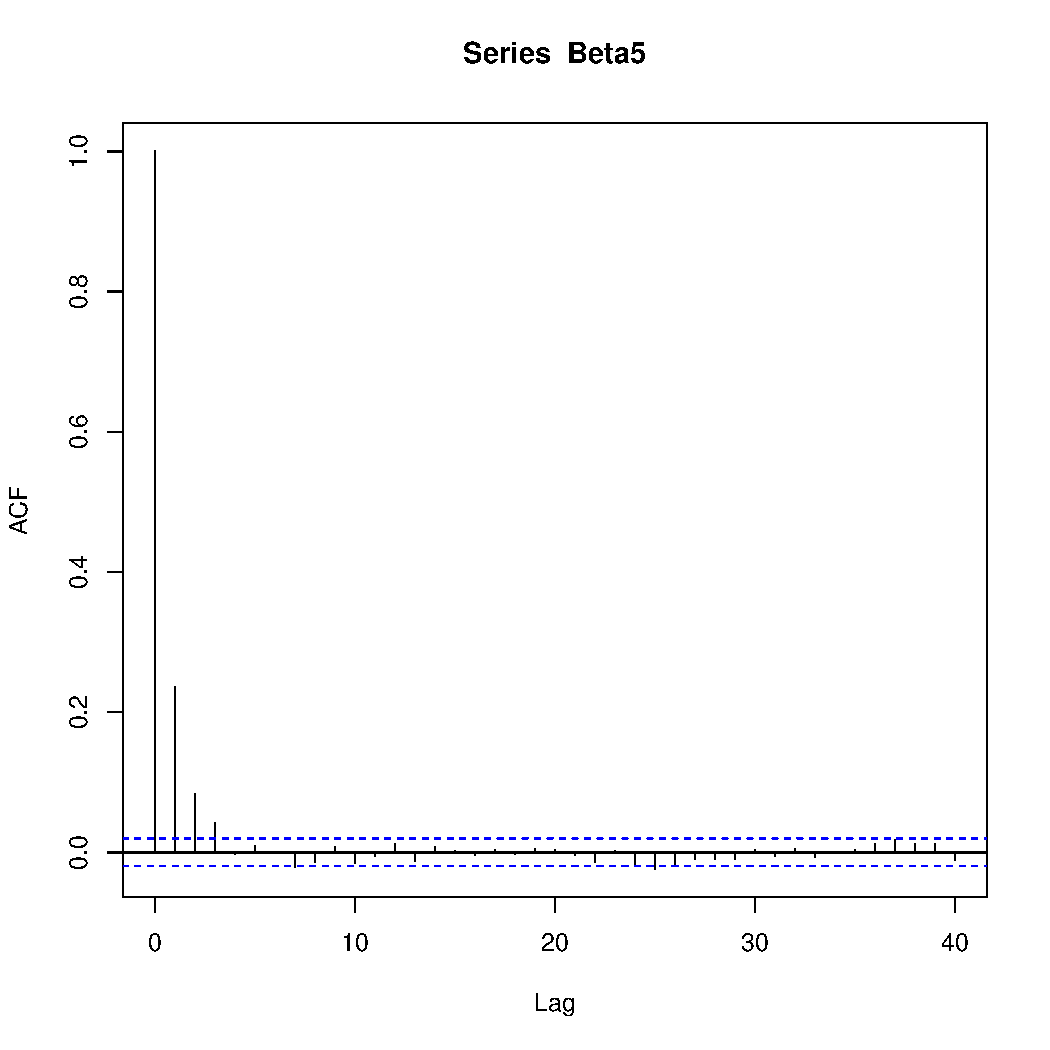
\includegraphics[width=0.7\textwidth]{Beta5ACFunsub.pdf}
  \caption{The sample auto-correlation function for the fifth covariate shows significant correlation at low lags. The dashed lines represent a 95\% confidence interval which should capture 95\% of correlations under the assumption of uncorrelated data.}
\end{figure}

To alleviate this issue a sub-sample of Gibbs samples were taken, wherein the sampling was repeated $5 \times 10,000$ times and only every fifth sample was kept. This produced a sample that was of size $n=10,000$, and when reassessing the sample size and autocorrelation all previous issues had vanished.

While having an uncorrelated Gibbs sample is preferred, the results found after adjusting the sampler did not differ in any meaningful way. In the end it would be more suitable to just take a larger sample size rather than a sub-sample to save the information gained for the less correlated variables.

\subsection{Convergence Paths}
When working with penalized regression of any sort, it is important to consider the entire path of estimates as the penalties vary. Figure~\ref{convergence} shows exactly that, allowing us to compare the Bayesian Lasso, Lasso, and Ridge Regression. 

As was noted in the paper by \cite{park2008bayesian}, and made slightly more obvious by the plotting approach taken here, Bayesian Lasso estimates appear to compromise between the Lasso and Ridge Regression estimates. This does not hold for the seventh covariate (good cholesterol levels) but does hold in most cases where the Lasso and Ridge Regression estimates differ. I WANT TO LOOK INTO WHY THIS IS MORE BUT IM NOT REALLY QUITE SURE

ALSO THE STUPID DASHED LINE MAKES NO SENSE, IT TORMENTS ME (Seriously though, it doesn't even match the n-fold cv lasso selected in the other plot... Why do you vex me so, glmnet)

\begin{figure}\label{convergence}
  \centering
    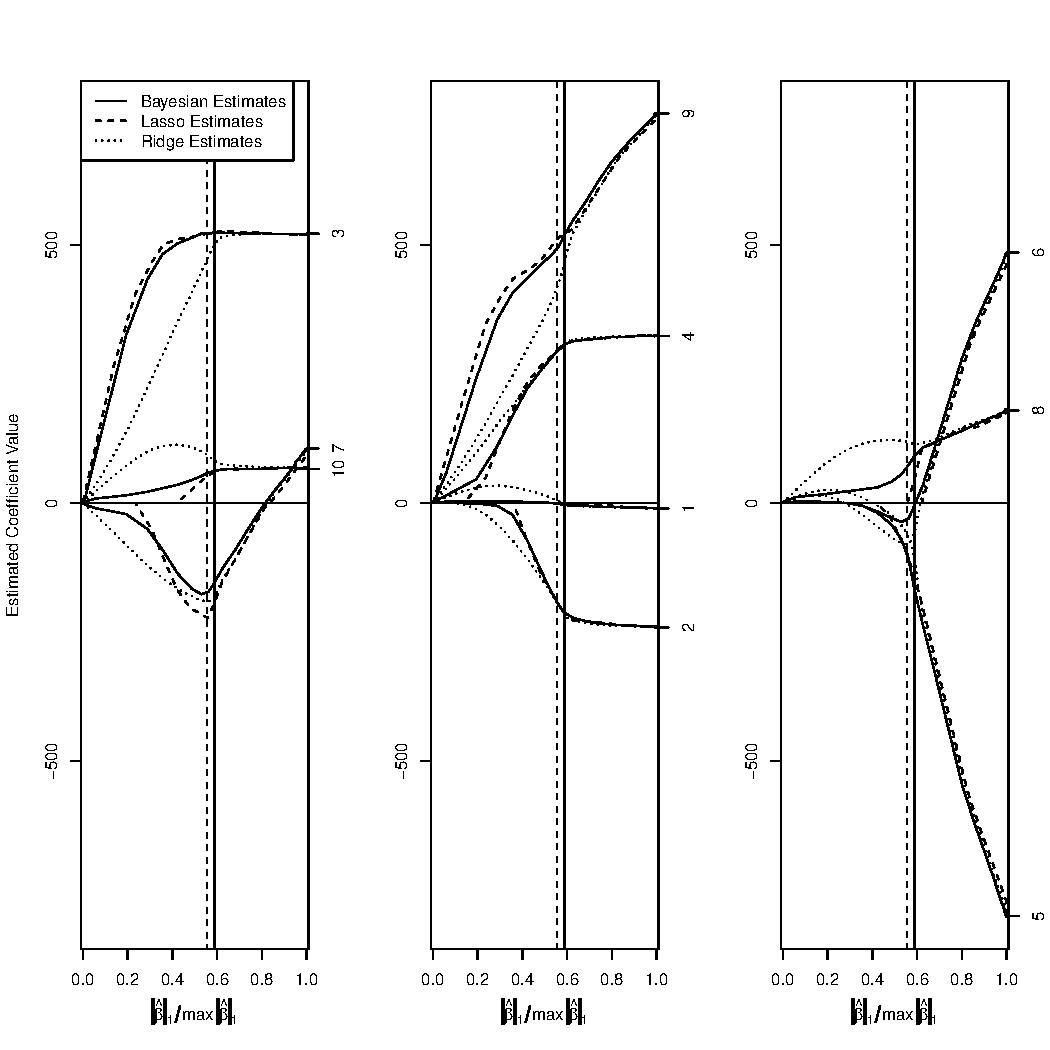
\includegraphics[width=0.7\textwidth]{SaveFigure1.pdf}
  \caption{Shown here are the convergence paths for the Bayesian Lasso, Lasso, and Ridge Regression. The horizontal lines represent values selected via Marginal Maximum Likelihood for the Bayesian Lasso and n-fold cross-validation in the case of the Lasso estimates. Variables have been separated into three plots for visibility, while allowing easier comparison of the three selection schemes.}
\end{figure}

\subsection{Credible Intervals}
While convergence is important, it is only looking at point estimates which were not the intent of the Bayesian Lasso. To get a more clear picture we turn to the parameter credible intervals. 

Figure~\ref{CIs} shows exactly that, with equal-tailed 95\% credible intervals on each of the parameters. As with the original paper, these were checked with $\lambda$ set via marginal maximum likelihood and hyperprior. In each case the results were indistinguishable from one another, and indistinguishable from the original results.

The first point that is important to note is that the n-fold ($\bigtriangleup$) and matched $L_1$ norm estimates ($\bigtriangledown$) both fall well within the credible intervals. Also the $L_1$ norm matched estimates (very akin to selecting for the same $\lambda$ value) are almost identical to the Bayesian Lasso estimates. 

\begin{figure}\label{CIs}
  \centering
    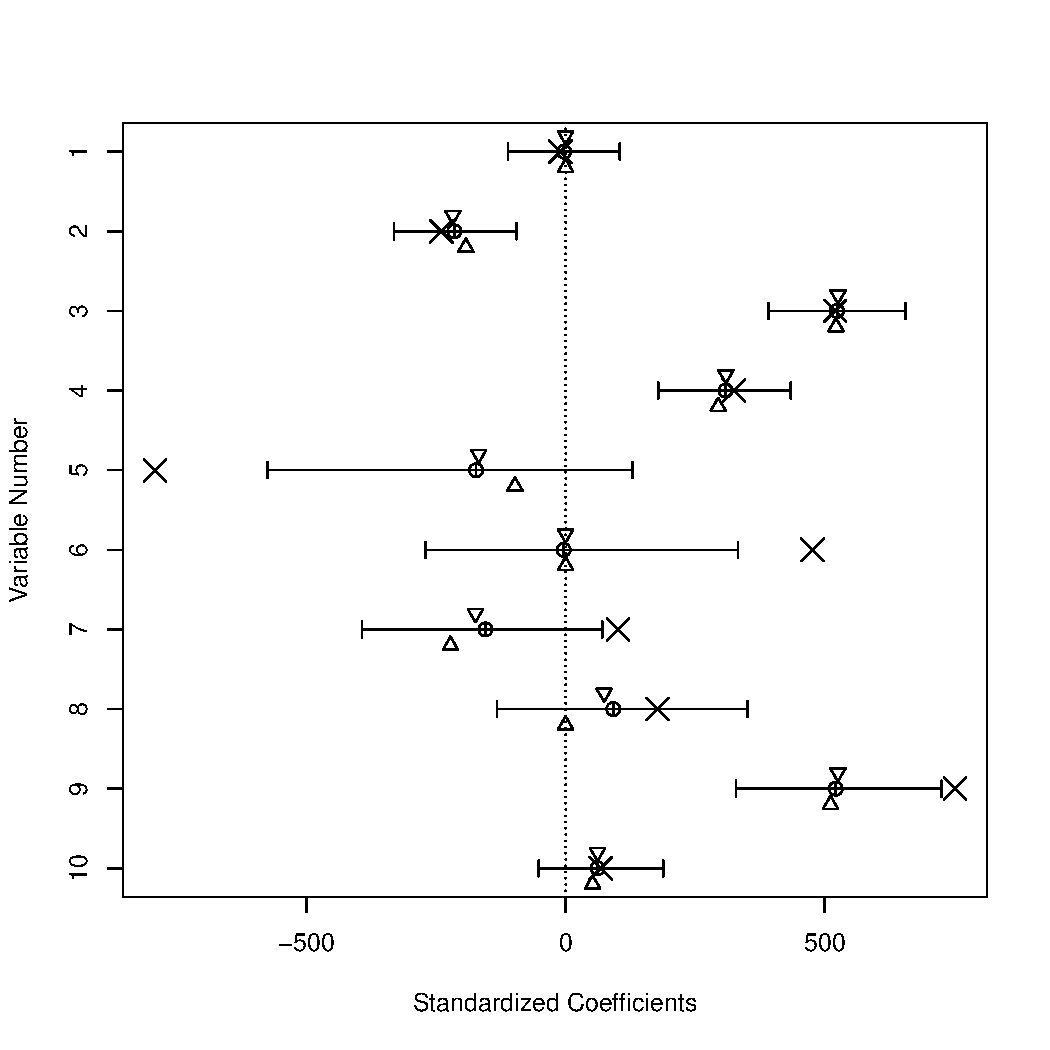
\includegraphics[width=0.7\textwidth]{SaveFigure2.pdf}
  \caption{Credible intervals are shown for each of the ten parameters, (1) age, (2) sex, (3) bmi, (4) map, and blood serum measures, (5) tc, (6) ldl, (7) hdl, (8) tch, (9) ltg, and (10) glu. Also marked are median Bayesian estimates ($\oplus$), Lasso estimates chosen to match the $L_1$ norm of Bayesian estimates ($\bigtriangledown$), Lasso estimates chosen by n-fold cross validation ($\bigtriangleup$), and lastly ordinary least squares estimates ($\times$).}
\end{figure}

\subsection{Hyperparameter Selection}
Selection of the hyperparameter $\lambda$ is an important choice when working with the Lasso. Marginal maximum likelihood offers us a data driven approach, while a Bayesian hyperprior fits will with our Bayesian approach and fits effortlessly into the Gibbs sampling scheme.

For selection of the marginal maximum likelihood, the original work cited an estimate for $\lambda$ of 0.237. In my own work I found, as shown in Figure~\ref{lambda}, that after extended sampling, values randomly deviated around a value slightly lower but not significantly different in the context of the greater problem.

\begin{figure}\label{lambda}
  \centering
    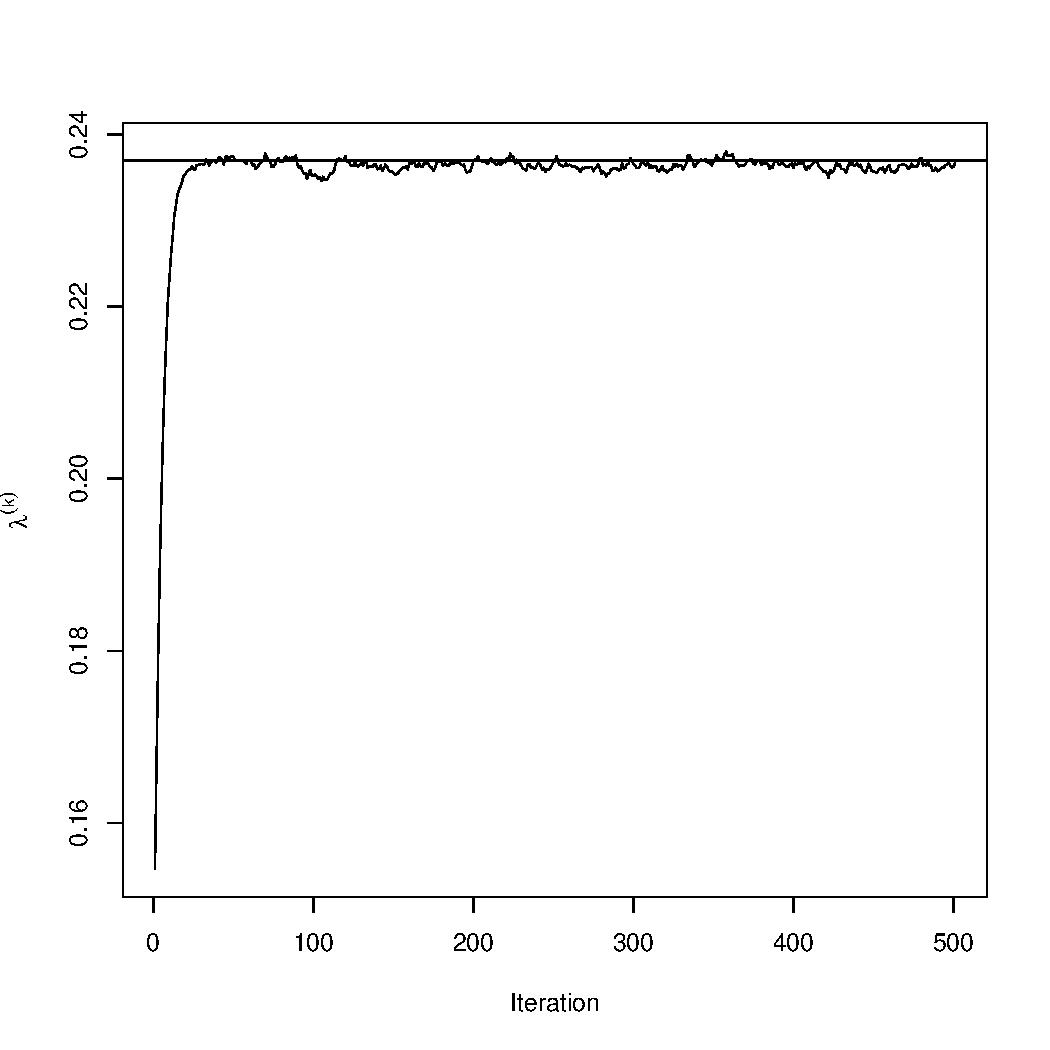
\includegraphics[width=0.7\textwidth]{SaveLambdaConverge.pdf}
  \caption{Shown here is the convergence of the marginal maximum likelihood estimate of $\lambda$. The horizontal line represents the estimate used by \cite{park2008bayesian} (.237) while the value found taking the last 900 of 1000 samples was .2365, not significantly different.}
\end{figure}

The selection via hyperprior gave similar results, and due to ease of computation was repeated for both the regular Gibbs sampler and the uncorrelated Gibbs sampler. In the original case, the sample of $\lambda$ had a median of .279 with a 95\% credible interval from 0.141 to 0.477. With the uncorrelated sampler the median was 0.274 with an interval from 0.141 to 0.483. This also further demonstrates the lack of need for the uncorrelated sampler.

\section{Discussion}

\bibliography{stat572}

\end{document}









